\section{Requisitos del sistema a desarrollar}


 \begin{figure}[H]
 \centering
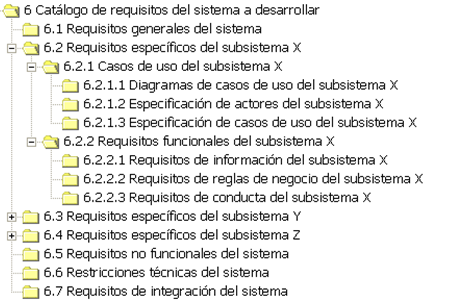
\includegraphics[width=0.8\textwidth]{\fig/indice.png}
 \caption{Ejemplo del índice}
 \end{figure}
 

\subsection{Requisitos Generales del Sistema [Opcional]}


 \begin{textoazul}
 Esta sección debe contener la especificación de los requisitos generales del sistema, también denominados características del sistema (system features) u objetivos del sistema, especificados mediante las  plantillas para requisitos generales que se muestran a continuación.
 

Los requisitos generales puede que ya se encuentren alineados con los objetivos del negocio. En el caso de que se considere necesario, los requisitos generales se podrán descomponer jerárquicamente para facilitar su comprensión.

\end{textoazul}

 \begin{Artefacto}[H]
    \centering
    \begin{tabular}{|p{3cm}|p{10cm}|}
        \hline
         \cellcolor{gray30}  REQ-GEN 999	&  $<nombre descriptivo>$\\ 
%      \cellcolor{gray30}  REQ-GEN 999	& <descriptive name>\\   
        \hline
         \cellcolor{gray30}  [Versión]	&  $<num version(fecha de version>$)\\   
%      \cellcolor{gray30}  [Version]	&   $<num version(date>$)\\   
         \hline
         \cellcolor{gray30}  [Dependencias] &  	\begin{itemize} 	\item $<requisito general padre, si lo tiene (padre)>$
\item $<otros requisitos generales de los que dependa>$
\item	... \end{itemize}\\  
%                 \cellcolor{gray30}  [Dependencies] &  	\begin{itemize} \item requirement
%\item	... \end{itemize}\\            
        \hline
         \cellcolor{gray30} Descripción	& $<descripcion>$  \\
%      \cellcolor{gray30}   Description	& \\   
          \hline
         \cellcolor{gray30}  Requisitos hijos&  	\begin{itemize} 	\item  
\item 
\item	... \end{itemize}\\  
%                 \cellcolor{gray30}  [Dependencies] &  	\begin{itemize} \item requirement
%\item	... \end{itemize}\\            
        \hline          
           \cellcolor{gray30}[Importancia]	& $<importancia para el cliente>$  \\
%      \cellcolor{gray30}   [Importance] 	& descrip\\   
         \hline
         \cellcolor{gray30}  [Prioridad] &  	$<prioridad para la direccion del proyecto>$\\
%                 \cellcolor{gray30}  [Priority] &   	\\  
         \hline
         \cellcolor{gray30}  [Estado]	&$<estado del requisito segun el ciclo de vida $ $ adoptado por el proyecto>$\\   
%         \cellcolor{gray30} State	&$<state according the lifecicle>$
        \hline       
         \cellcolor{gray30}  Comentarios	&$<comentarios adicionales $\\   
%         \cellcolor{gray30} Comments	&$<additional comments>$
        \hline
  
    \end{tabular}
\caption{REQ-GEN 999	$<nombre descriptivo>$ }
%\caption{REQ-GEN 999	$<descriptive name >$ }
  \end{Artefacto}



\subsection{Casos de uso del Sistema}
\begin{textoazul}
 Esta sección debe contener la especificación de los casos de uso del sistema, denominados escenarios operacionales en terminología CMMI-DEV, incluyendo los correspondientes diagramas, la especificación de los actores y la especificación de los propios casos de uso. Los casos de uso deben describir cómo se utilizará el sistema a desarrollar por sus futuros usuarios para realizar sus procesos de negocio
\end{textoazul} 
 
\subsubsection{Diagramas de Casos de Uso del Sistema}

 
  \begin{figure}[H]
\centering
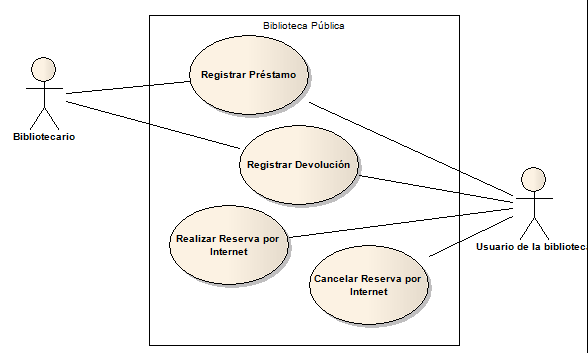
\includegraphics[width=0.8\textwidth]{\fig/casos.png}
\caption{Ejemplo del diagrama de casos de uso}
\end{figure}



\subsubsection{Especificación de Actores del Sistema}
<Introduzca contenido, cumplimente tabla y borre cuadro>

  \begin{Artefacto}[H]
    \centering
    \begin{tabular}{|p{3cm}|p{10cm}|}
        \hline
         \cellcolor{gray30}  CDU-ACT 999	&  $<nombre descriptivo>$\\ 
%      \cellcolor{gray30}  CDU-ACT 999	& <descriptive name>\\   
        \hline
         \cellcolor{gray30}  [Versión]	&  $<num version(fecha de version>$)\\   
%      \cellcolor{gray30}  [Version]	&   $<nº version>$($<date>$)\\   
         \hline
         \cellcolor{gray30}  [Dependencias] &  	\begin{itemize} \item $<actores del negocio relacionados>$\item	... \end{itemize}\\  

%                 \cellcolor{gray30}  [Dependencies] &  	\begin{itemize} \item $<related business actors>$
%\item	... \end{itemize}\\            
        \hline
         \cellcolor{gray30} Descripción	& $<descripcion del rol que representa el actor en$ $ los casos de uso del sistema >$ \\
%      \cellcolor{gray30}   Description	& descrip\\   
        \hline
         \cellcolor{gray30}  Comentarios	&$<comentarios adicionales sobre el actor de negocio  a$ $ implantar>$\\   
%         \cellcolor{gray30} Comments	&$<additional comments>$
        \hline
  
    \end{tabular}
\caption{CDU-ACT 999	$<nombre descriptivo>$ }
%\caption{CDU-ACT 999	$<descriptive name >$ }
  \end{Artefacto}



\subsubsection{Especificación de Casos de Uso del Sistema}


 


\begin{Artefacto}[H]
    \centering
    \begin{tabular}{|p{3cm}|p{10cm}|}
        \hline
         \cellcolor{gray30}  CDU-999	&  $<nombre descriptivo>$\\ 
%      \cellcolor{gray30}  REQ-GEN 999	& <descriptive name>\\   
        \hline
         \cellcolor{gray30}  [Versión]	&  $<num version(fecha de version>$)\\   
%      \cellcolor{gray30}  [Version]	&   $<num version>$($<date>$)\\   
         \hline
         \cellcolor{gray30}  [Dependencias] &  	\begin{itemize} 	\item $<requisitos generales de los que depende>$
\item $<otros requisitos generales de los que dependa>$
\item	... \end{itemize}\\  
%                 \cellcolor{gray30}  [Dependencies] &  	\begin{itemize} \item requirement
%\item	... \end{itemize}\\            
        \hline
         \cellcolor{gray30} Descripción	&El sistema deberá comportarse tal como se indica en la siguiente especificación del caso de uso\\
%      \cellcolor{gray30}   Description	& descrip\\   
\hline
          
         \cellcolor{gray30}  Secuencia normal&  	
         \begin{enumerate} 	
             \item	{El actor $<$actor del sistema$>$, El sistema}<acción/es realizada/s por el actor del sistema>
			\item	Se realiza el $<$caso de uso del sistema$>$
			\item	Si <condición>,
            ...	...
            \begin{enumerate}
		       \item El caso de uso termina con éxito,Se cancela el caso de uso
               \item
       
        	\end{enumerate}
	...	...\item paso 
													
       \item	... \end{enumerate}\\  

\hline          
  \cellcolor{gray30} Postcondición	& postcondición del caso de uso del sistema \\
  \hline
 \cellcolor{gray30}  Excepciones&
 \begin{itemize} 	        
			\item	$<$PASO m$>$	Si $<$condición de excepción$>$
            \begin {enumerate}
            \item 	{El caso de uso continua,Se cancela el caso de uso}
            \item
            \end{enumerate}
            \item	$<$PASO n$>$: 
 \end{itemize}\\ 
\hline
        \hline          
           \cellcolor{gray30}[Importancia]	& $<importancia del requisito para el cliente>$  \\
%      \cellcolor{gray30}   Importance 	& descrip\\   
         \hline
         \cellcolor{gray30}  [Prioridad] &  	$<prioridad del requisito para la direccion del proyecto>$\\
%                 \cellcolor{gray30}  [Priority] &   	\\  
         \hline
         \cellcolor{gray30}  Estado	&$<estado  segun el ciclo de vida adoptado por el proyecto>>$\\   
%         \cellcolor{gray30} State	&$<state according the lifecicle>$
        \hline       
         \cellcolor{gray30}  Comentarios	& $<comentarios adicionales>$ \\   
%         \cellcolor{gray30} Comments	&$<additional comments>$
        \hline
  
    \end{tabular}
\caption{CDU 999	$<nombre descriptivo>$ }
%\caption{CDU 999	$<descriptive name >$ }
  \end{Artefacto}











\subsection{Requisitos Funcionales del Sistema}

\begin{textoazul}
Esta sección debe contener los requisitos funcionales del sistema que se hayan identificado a partir de los requisitos generales, de los casos de uso del sistema o de otras fuentes. Se divide en las secciones que se describen a continuación.
\end{textoazul}
  

            
\subsubsection{Requisitos de Información del Sistema}
<Introduzca contenido, cumplimente tabla y borre cuadro>
 
 
   \begin{figure}[H]
 \centering
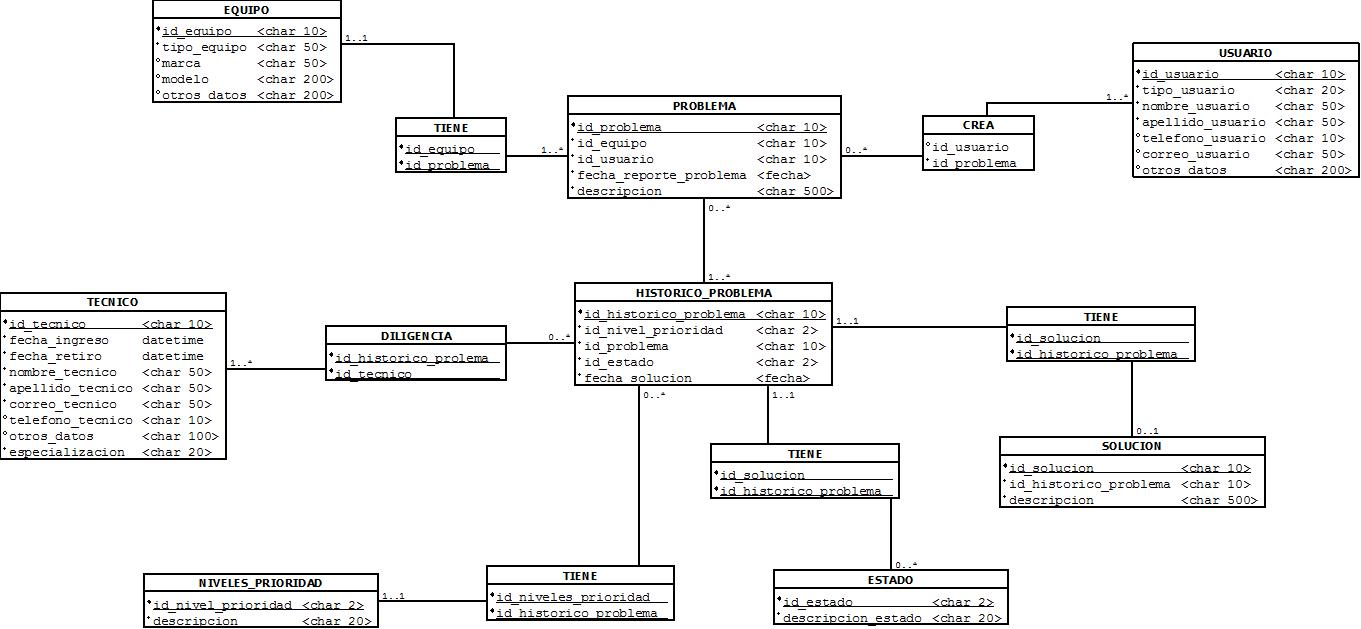
\includegraphics[width=0.8\textwidth]{\fig/datos.jpg}
 \caption{Ejemplo de modelo de datos}
 \end{figure}
 



\begin{Artefacto}[H]
    \centering
    \begin{tabular}{|p{3cm}|p{10cm}|}
        \hline
         \cellcolor{gray30}  REQ-GEN 999	&  $<nombre descriptivo>$\\ 
%      \cellcolor{gray30}  REQ-GEN 999	& <descriptive name>\\   
        \hline
         \cellcolor{gray30}  [Versión]	&  $<num version(fecha de version>$)\\   
%      \cellcolor{gray30}  [Version]	&   $<num version>$($<date>$)\\   
         \hline
         \cellcolor{gray30}  [Dependencias] &  	\begin{itemize} 	\item $<requisitos generales de los que depende>$
\item $<otros requisitos generales de los que dependa>$
\item	... \end{itemize}\\  
%                 \cellcolor{gray30}  [Dependencies] &  	\begin{itemize} \item requirement
%\item	... \end{itemize}\\            
        \hline
         \cellcolor{gray30} Descripción	&El sistema deberá almacenar la información correspondiente a <concepto relevante>. En concreto:\\
%      \cellcolor{gray30}   Description	& descrip\\   
          \hline
         \cellcolor{gray30}  Datos específicos&  	\begin{itemize} 	\item dato: tipo
                                                                                           \item 
																	\item	... \end{itemize}\\  
%                 \cellcolor{gray30}  [Dependencies] &  	\begin{itemize} \item requirement
%\item	... \end{itemize}\\            
        \hline          
           \cellcolor{gray30}[Importancia]	& $<importancia del requisito para el cliente>$  \\
%      \cellcolor{gray30}   Importance 	& descrip\\   
         \hline
         \cellcolor{gray30}  [Prioridad] &  	$<prioridad del requisito para la direccion del proyecto>$\\
%                 \cellcolor{gray30}  [Priority] &   	\\  
         \hline
         \cellcolor{gray30}  Estado	&$<estado  segun el ciclo de vida adoptado por el proyecto>>$\\   
%         \cellcolor{gray30} State	&$<state according the lifecicle>$
        \hline       
         \cellcolor{gray30}  Comentarios	& $<comentarios adicionales>$ \\   
%         \cellcolor{gray30} Comments	&$<additional comments>$
        \hline
  
    \end{tabular}
\caption{REQ-INF 999	$<nombre descriptivo>$ }
%\caption{REQ-INF 999	$<descriptive name >$ }
  \end{Artefacto}






\subsection{Requisitos No Funcionales del Sistema}




\begin{Artefacto}[H]
    \centering
    \begin{tabular}{|p{3cm}|p{10cm}|}
        \hline
         \cellcolor{gray30}  REQ-GEN 999	&  $<nombre descriptivo>$\\ 
%      \cellcolor{gray30}  REQ-GEN 999	& <descriptive name>\\   
        \hline
         \cellcolor{gray30}  [Versión]	&  $<num version(fecha de version>$)\\   
%      \cellcolor{gray30}  [Version]	&   $<num version>$($<date>$)\\   
         \hline
         \cellcolor{gray30}  [Dependencias] &  	\begin{itemize} 	\item $<requisitos generales de los que depende>$
\item $<otros requisitos generales de los que dependa>$
\item	... \end{itemize}\\  
%                 \cellcolor{gray30}  [Dependencies] &  	\begin{itemize} \item requirement
%\item	... \end{itemize}\\            
        \hline
         \cellcolor{gray30} Descripción	&El sistema deberá  $<descripcion no funcional del sistema>$\\
%      \cellcolor{gray30}   Description	& descrip\\   
          \hline
         \cellcolor{gray30}  Requisitos hijos&  	\begin{itemize} 	\item 
                                                                                           \item 
																	\item	... \end{itemize}\\  
%                 \cellcolor{gray30}  [Dependencies] &  	\begin{itemize} \item requirement
%\item	... \end{itemize}\\            
        \hline          
           \cellcolor{gray30}[Importancia]	& $<importancia del requisito para el cliente>$  \\
%      \cellcolor{gray30}   Importance 	& descrip\\   
         \hline
         \cellcolor{gray30}  [Prioridad] &  	$<prioridad del requisito para la direccion del proyecto>$\\
%                 \cellcolor{gray30}  [Priority] &   	\\  
         \hline
         \cellcolor{gray30}  Estado	&$<estado  segun el ciclo de vida adoptado por el proyecto>>$\\   
%         \cellcolor{gray30} State	&$<state according the lifecicle>$
        \hline       
         \cellcolor{gray30}  Comentarios	& $<comentarios adicionales>$ \\   
%         \cellcolor{gray30} Comments	&$<additional comments>$
        \hline
  
    \end{tabular}
\caption{RNF-$<tipo>$ 999	$<nombre descriptivo>$ }
%\caption{REQ-INT 999	$<descriptive name >$ }
  \end{Artefacto}




\subsubsection{Requisitos de Fiabilidad}

 
\subsubsection{Requisitos de Usabilidad}

 
\subsubsection{Requisitos de Eficiencia}

 
\subsubsection{Requisitos de Mantenibilidad}

 
\subsubsection{Requisitos de Portabilidad}

 
\subsubsection{Requisitos de Seguridad}

 
\subsubsection{Otros Requisitos No Funcionales}

 

\subsection{Restricciones Técnicas del Sistema}


 \begin{Artefacto}[H]
    \centering
    \begin{tabular}{|p{3cm}|p{10cm}|}
        \hline
         \cellcolor{gray30}  REQ-GEN 999	&  $<nombre descriptivo>$\\ 
%      \cellcolor{gray30}  REQ-GEN 999	& <descriptive name>\\   
        \hline
         \cellcolor{gray30}  [Versión]	&  $<num version(fecha de version>$)\\   
%      \cellcolor{gray30}  [Version]	&   $<num version(date>$)\\   
         \hline
         \cellcolor{gray30}  [Dependencias] &  	\begin{itemize} 	\item requisitos generales de los que depende
\item otros requisitos generales de los que dependa
\item	... \end{itemize}\\  
%                 \cellcolor{gray30}  [Dependencies] &  	\begin{itemize} \item requirement
%\item	... \end{itemize}\\            
        \hline
         \cellcolor{gray30} Descripción	&El sistema deberá respetar la siguiente restricción técnica: $<descripcion de la restriccion tecnica del sistema>$  \\
%      \cellcolor{gray30}   Description	& descrip\\   
          \hline
         \cellcolor{gray30}  Requisitos hijos&  	\begin{itemize} 	\item requisito 
\item otros requisitos 
\item	... \end{itemize}\\  
%                 \cellcolor{gray30}  [Dependencies] &  	\begin{itemize} \item requirement
%\item	... \end{itemize}\\            
        \hline          
           \cellcolor{gray30}`[Importancia]	& $<importancia de la restriccion tecnica para el cliente>$  \\
%      \cellcolor{gray30}   Importance 	& descrip\\   
         \hline
         \cellcolor{gray30}  [Prioridad] &  	$<prioridad para la direccion del proyecto>$\\
%                 \cellcolor{gray30}  [Priority] &   	\\  
         \hline
         \cellcolor{gray30}  Estado	&$<estado segun el ciclo de vida adoptado por el proyecto>$\\   
%         \cellcolor{gray30} State	&$<state according the lifecycle>$
        \hline       
         \cellcolor{gray30}  Comentarios	&$<comentarios adicionales >$\\   
%         \cellcolor{gray30} Comments	&$<additional comments>$
        \hline
  
    \end{tabular}
\caption{REQ-REST 999	$<nombre descriptivo>$ }
%\caption{REQ-CON 999	$<descriptive name >$ }
  \end{Artefacto}



 


\subsection{Requisitos de Integración del Sistema}

 



 \begin{Artefacto}[H]
    \centering
    \begin{tabular}{|p{3cm}|p{10cm}|}
        \hline
         \cellcolor{gray30}  REQ-GEN 999	&  $<nombre descriptivo>$\\ 
%      \cellcolor{gray30}  REQ-GEN 999	& <descriptive name>\\   
        \hline
         \cellcolor{gray30}  [Versión]	&  $<num version(fecha de version>$)\\   
%      \cellcolor{gray30}  [Version]	&   $<num version(date>$)\\   
         \hline
         \cellcolor{gray30}  [Dependencias] &  	\begin{itemize} 	\item requisitos generales de los que depende
\item otros requisitos generales de los que dependa
\item	... \end{itemize}\\  
%                 \cellcolor{gray30}  [Dependencies] &  	\begin{itemize} \item requirement
%\item	... \end{itemize}\\            
        \hline
         \cellcolor{gray30} Descripción	&El sistema deberá utilizar el {servicio, componente software} $<nombre del elemento a integrar>$ para aquellos aspectos relacionados con $<funcionalidad prestada por el elemento a integrar>$ \\
%      \cellcolor{gray30}   Description	& descrip\\   
          \hline
         \cellcolor{gray30}  Requisitos hijos&  	\begin{itemize} 	\item requisito 
\item otros requisitos 
\item	... \end{itemize}\\  
%                 \cellcolor{gray30}  [Dependencies] &  	\begin{itemize} \item requirement
%\item	... \end{itemize}\\            
        \hline          
           \cellcolor{gray30}Importancia	& $<importancia del requisito para el cliente>$  \\
%      \cellcolor{gray30}   Importance 	& descrip\\   
         \hline
         \cellcolor{gray30}  [Prioridad] &  	$<prioridad del requisito para la direccion del proyecto>$\\
%                 \cellcolor{gray30}  [Priority] &   	\\  
         \hline
         \cellcolor{gray30}  Estado	&$<estado  segun el ciclo de vida adoptado por el proyecto>>$\\   
%         \cellcolor{gray30} State	&$<state according the lifecicle>$
        \hline       
         \cellcolor{gray30}  Comentarios	& $<comentarios adicionales>$ \\   
%         \cellcolor{gray30} Comments	&$<additional comments>$
        \hline
  
    \end{tabular}
\caption{REQ-INT 999	$<nombre descriptivo>$ }
%\caption{REQ-INT 999	$<descriptive name >$ }
  \end{Artefacto}




\subsection{Información Sobre Trazabilidad}

\begin{textoazul}
Esta sección obligatoria debe contener el conjunto de matrices de trazabilidad que se considere oportuno para identificar las relaciones entre los requisitos identificados. Al menos deberá incluir la siguiente matriz:
\begin{itemize}
\item Matriz de trazabilidad de Requisitos Generales frente a Objetivos de Negocio.
\item Matriz de trazabilidad de Casos de Uso frente a Requisitos Generales.
\item Matriz de trazabilidad de Requisitos de Información frente a Requisitos Generales.
\item Matriz de trazabilidad de Reglas de Negocio frente  a Requisitos Generales.
\item Matriz de trazabilidad de Requisitos de Conducta frente a Requisitos Generales.
\item Matriz de trazabilidad de Requisitos no Funcionales frente a Requisitos Generales.
\item Matriz de trazabilidad de Restricciones Técnicas frente a Requisitos Generales.
\item Matriz de trazabilidad de Requisitos de Integración frente a Requisitos Generales.

\end{itemize}
\end{textoazul}
 

